\chapter{Dữ liệu và phương pháp}

\section{Nguồn và mô tả dữ liệu}
Dữ liệu là các bình luận đánh giá sản phẩm công khai trên website Điện Máy Xanh, được lưu trữ tại \code{data/raw/}. Bảng \ref{tab:rating-raw} tổng hợp phân bố rating thô; các số liệu này mô tả dữ liệu crawl trước bước lọc và khử trùng lặp.

\begin{table}[H]
\centering
\caption{Phân bố rating trên 12.189 dòng thô}
\label{tab:rating-raw}
\begin{tabular}{lrr}
\toprule
Rating & Số mẫu & Tỷ lệ \\
\midrule
1 sao & 1.347 & 11,05\% \\
2 sao & 706 & 5,79\% \\
3 sao & 988 & 8,11\% \\
4 sao & 2.407 & 19,75\% \\
5 sao & 6.741 & 55,30\% \\
\midrule
Tổng & 12.189 & 100,00\% \\
\bottomrule
\end{tabular}
\end{table}

Các nhóm sản phẩm chính gồm tủ lạnh (3.366 dòng), nồi cơm điện (2.796), máy lạnh (2.030), máy giặt (1.725), máy lọc nước (1.724) và tivi (548). Phân bố rating lệch về 4--5 sao, vì vậy phân loại theo rating trực tiếp có thể tạo mất cân bằng lớp và không luôn phản ánh đúng nội dung văn bản.

\begin{figure}[H]
  \centering
  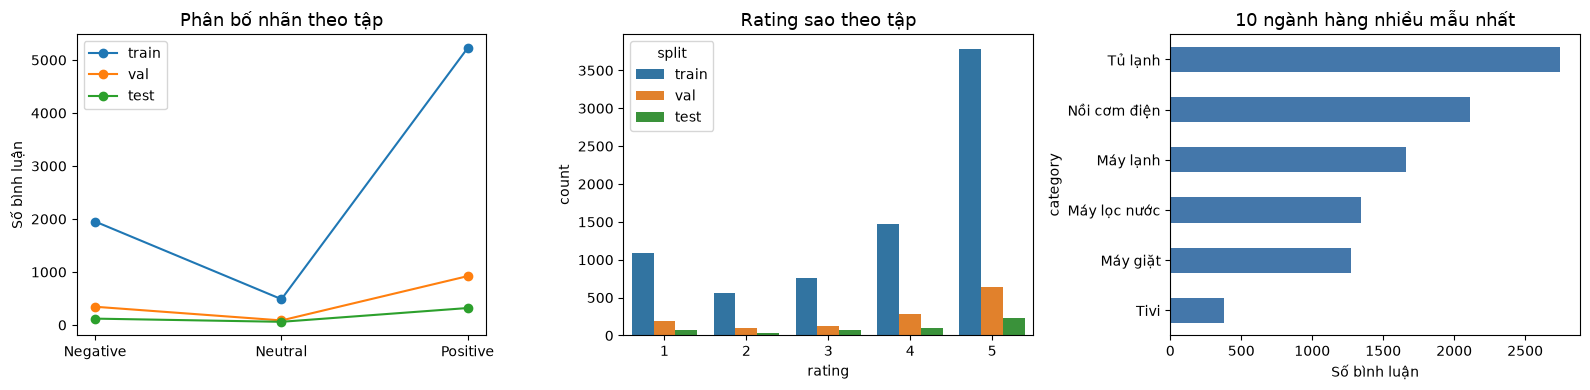
\includegraphics[width=\textwidth]{eda_data_overview.png}
  \caption{Tổng quan dữ liệu: phân bố nhãn theo split, rating theo split và số mẫu theo ngành hàng.}
  \label{fig:data-overview}
\end{figure}

\section{Làm sạch và tiền xử lý}
Quy trình xử lý được cài tại \code{src/data/preprocess.py} và gồm:
\begin{enumerate}
  \item bỏ nội dung rỗng, dạng lặp/ký tự vô nghĩa và bản ghi trùng theo cặp nội dung--rating;
  \item chuẩn hóa Unicode NFC, chữ thường, URL/HTML, teencode và một số lỗi chính tả/không dấu thường gặp;
  \item tách từ tiếng Việt bằng PyVi/Underthesea khi có sẵn, hoặc fallback miền thiết bị;
  \item tạo \code{text_segmented} cho PhoBERT (giữ cấu trúc và stopword) và \code{text_clean} cho ML cổ điển (lọc stopword nhưng bảo toàn phủ định/cảm xúc).
\end{enumerate}
Trong lần chạy hiện có, 49 dòng rác và 2.624 dòng trùng lặp bị loại; còn 9.516 review duy nhất hợp lệ.

\section{Gán nhãn hybrid và xử lý mâu thuẫn}
Nhãn sao ban đầu ánh xạ 1--2 sao thành Negative, 3 sao thành Neutral và 4--5 sao thành Positive. Bộ chấm lexicon miền thiết bị tại \code{src/data/auto_labeler.py} tính cực tính từ các từ tích cực/tiêu cực, điều chỉnh theo phủ định, cường độ và mệnh đề chuyển ý. Khi score văn bản mâu thuẫn mạnh với rating, quy tắc reconciliation có thể điều chỉnh nhãn đích. Quy trình lưu đồng thời \code{label_star}, \code{label_unsup}, \code{confidence}, \code{conflict_type} và \code{label_target} để có thể kiểm tra.

Trong 9.516 review hợp lệ, phân bố nhãn sao ban đầu là Negative 2.051 (21,55\%), Neutral 953 (10,01\%), Positive 6.512 (68,43\%). Sau reconciliation, nhãn đích là Negative 2.415 (25,38\%), Neutral 633 (6,65\%), Positive 6.468 (67,97\%). Có 490 trường hợp conflict được lưu để rà soát: 294 review ba sao có phàn nàn rõ; 79 review bốn--năm sao có nội dung tiêu cực mạnh; 67 review ba sao tích cực rõ; 41 review bốn sao pha trộn; và 9 review một--hai sao có nội dung tích cực.

\begin{figure}[H]
  \centering
  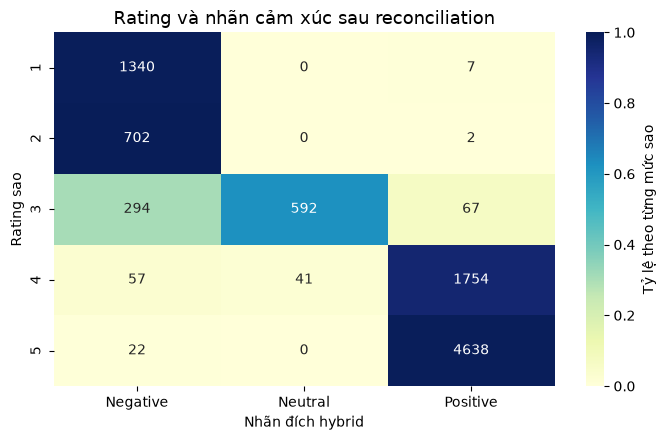
\includegraphics[width=0.78\textwidth]{rating_target_heatmap.png}
  \caption{Heatmap chéo giữa rating gốc và nhãn cảm xúc hybrid. Mỗi hàng được chuẩn hóa theo tỷ lệ rating; con số trong ô là số lượng mẫu.}
  \label{fig:rating-target}
\end{figure}

\begin{center}
\colorbox{softblue}{\parbox{0.92\textwidth}{\textbf{Giới hạn chất lượng nhãn.} Nhãn đích do quy tắc tự động tạo, chưa có đánh giá độc lập từ người gán. Vì vậy, các mô hình có thể học lại thiên lệch của lexicon/rating; chỉ số tại Chương 4 là mức đồng thuận với pseudo-label.}}
\end{center}

\section{Chia tập dữ liệu}
Dữ liệu được chia phân tầng theo \code{label_target} với seed 42. Các tập không có trùng lặp \code{review_id}. Split hiện tại là ngẫu nhiên theo review, không group theo mã sản phẩm; do đó cùng một sản phẩm có thể xuất hiện ở train và test.

\begin{table}[H]
\centering
\caption{Kích thước và phân bố nhãn của các split}
\label{tab:splits}
\begin{tabular}{lrrrr}
\toprule
Split & Tổng & Negative & Neutral & Positive \\
\midrule
Train & 7.664 & 1.951 & 487 & 5.226 \\
Validation & 1.352 & 344 & 86 & 922 \\
Held-out test & 500 & 120 & 60 & 320 \\
\bottomrule
\end{tabular}
\end{table}

Tập held-out được đặt tên \code{test.csv}, không dùng thuật ngữ ``gold test'' vì chưa gán thủ công. Vectorizer và Word2Vec chỉ fit trên train; validation phục vụ lựa chọn mô hình; test dùng đánh giá cuối.

\section{Thiết kế đặc trưng và mô hình}
\begin{table}[H]
\centering
\caption{Các nhánh thực nghiệm}
\label{tab:experiments}
\begin{tabularx}{\textwidth}{p{2.5cm}p{4.1cm}Y}
\toprule
Đặc trưng & Bộ phân loại & Mô tả cấu hình \\
\midrule
BoW & MultinomialNB, LinearSVC & CountVectorizer unigram/bigram, max 15.000 đặc trưng; NB $\alpha=1,0$, SVM $C=0,5$. \\
TF--IDF & MultinomialNB, LinearSVC & unigram/bigram, sublinear TF, max 15.000 đặc trưng; NB $\alpha=0,5$, SVM $C=1,0$. \\
Word2Vec & GaussianNB, LinearSVC & Skip-gram 100 chiều, window 5, min-count 2; vector câu mean pooling; SVM $C=1,0$. \\
Transformer & PhoBERT, XLM-R Large & Weighted cross-entropy, validation Macro-F1, early stopping; runner có sẵn nhưng chưa có kết quả fine-tune trong bảng hiện tại. \\
\bottomrule
\end{tabularx}
\end{table}
Naïve Bayes sử dụng hybrid resampling để giảm lệch lớp; SVM dùng trọng số lớp cân bằng. Majority baseline luôn dự đoán lớp có tần suất cao nhất.
